\subsubsection{概要}
しらたまチームで使用した自己位置推定のパッケージは, 
他チームと同じくemcl2\_ros2を使用した. 
本チームでは, 
ソースコードには手を入れず, 
パラメータのみを変更して使用した. 

ナビゲーションにはROS 2標準のパッケージであるnavigation2\cite{nav2}を使用した. 
このパッケージも同様にパラメータのみを変更して使用した. 

% しらたまチームは1章で述べた目標のために, 
% 上田研究室に保存されているドキュメントを用いてロボットのセットアップや実装を行った. 
% しらたまチームでは, 自己位置推定にemcl2\_ros2,ナビゲーションにnavigation2を採用した. 

%開発してないので省略
%\subsubsection{開発したパッケージ}

%システム図作成する必要あり
\subsubsection{システム構成}
ロボットに搭載した計算機, センサ, 
アクチュエータの接続の関係及び計算機で実行するROS 2ノードの概要を表したものを図\ref{fig:shiratama_system}に示す. 
Raspberry Piには, 車輪駆動用のモータと2D LiDARを接続した. 
実行するノードとしては, 
2D LiDAR用のROS 2ドライバノード(urg\_node)と, 
他チームでも使用しているraspimouseノードがある. 
本チームではエンコーダとIMUを搭載していないため, 
オドメトリは, 速度指令値を積分することで計算している. 

ノートPCでは, Raspberry Piからオドメトリと2D LiDARのトピックを受け取り, 
自己位置推定とナビゲーションの処理を実行する. 
実行するノードとしては, 
\begin{itemize} 
\item map\_server: 事前に作成した環境地図をトピックとして配信するノード. 
\item emcl2: モンテカルロ自己位置推定(MCL)を実行するノード. 
\item navigation2: ナビゲーションパッケージに属するノード(図中では複数のノードをまとめて「navigation2」と表記)
\end{itemize}
がある. 
emcl2ノードでは, map\_serverが配信する環境地図の情報を含んだトピック(図中の/map)を受け取る. 
この環境地図の作成には, ROS 2標準のSLAMパッケージであるslam\_toolbox\cite{slam_toolbox}を使用した. 

% \begin{itemize} 
% \item urg\_node: レーザにより周囲の障害物との距離を測定し,スキャンデータとして配信. 

% \item raspimouse: ロボットの駆動制御を行う. また,エンコーダの代わりに,速度指令値(cmd\_vel)をオドメトリの情報(/odom)として配信.

% \item map\_server: 事前に作成した環境地図を配信.

% \item emcl2: モンテカルロ自己位置推定(MCL)を実行するノード.
% \end{itemize}
% %something
% がある.  

\begin{figure}[h]
  \begin{center}
    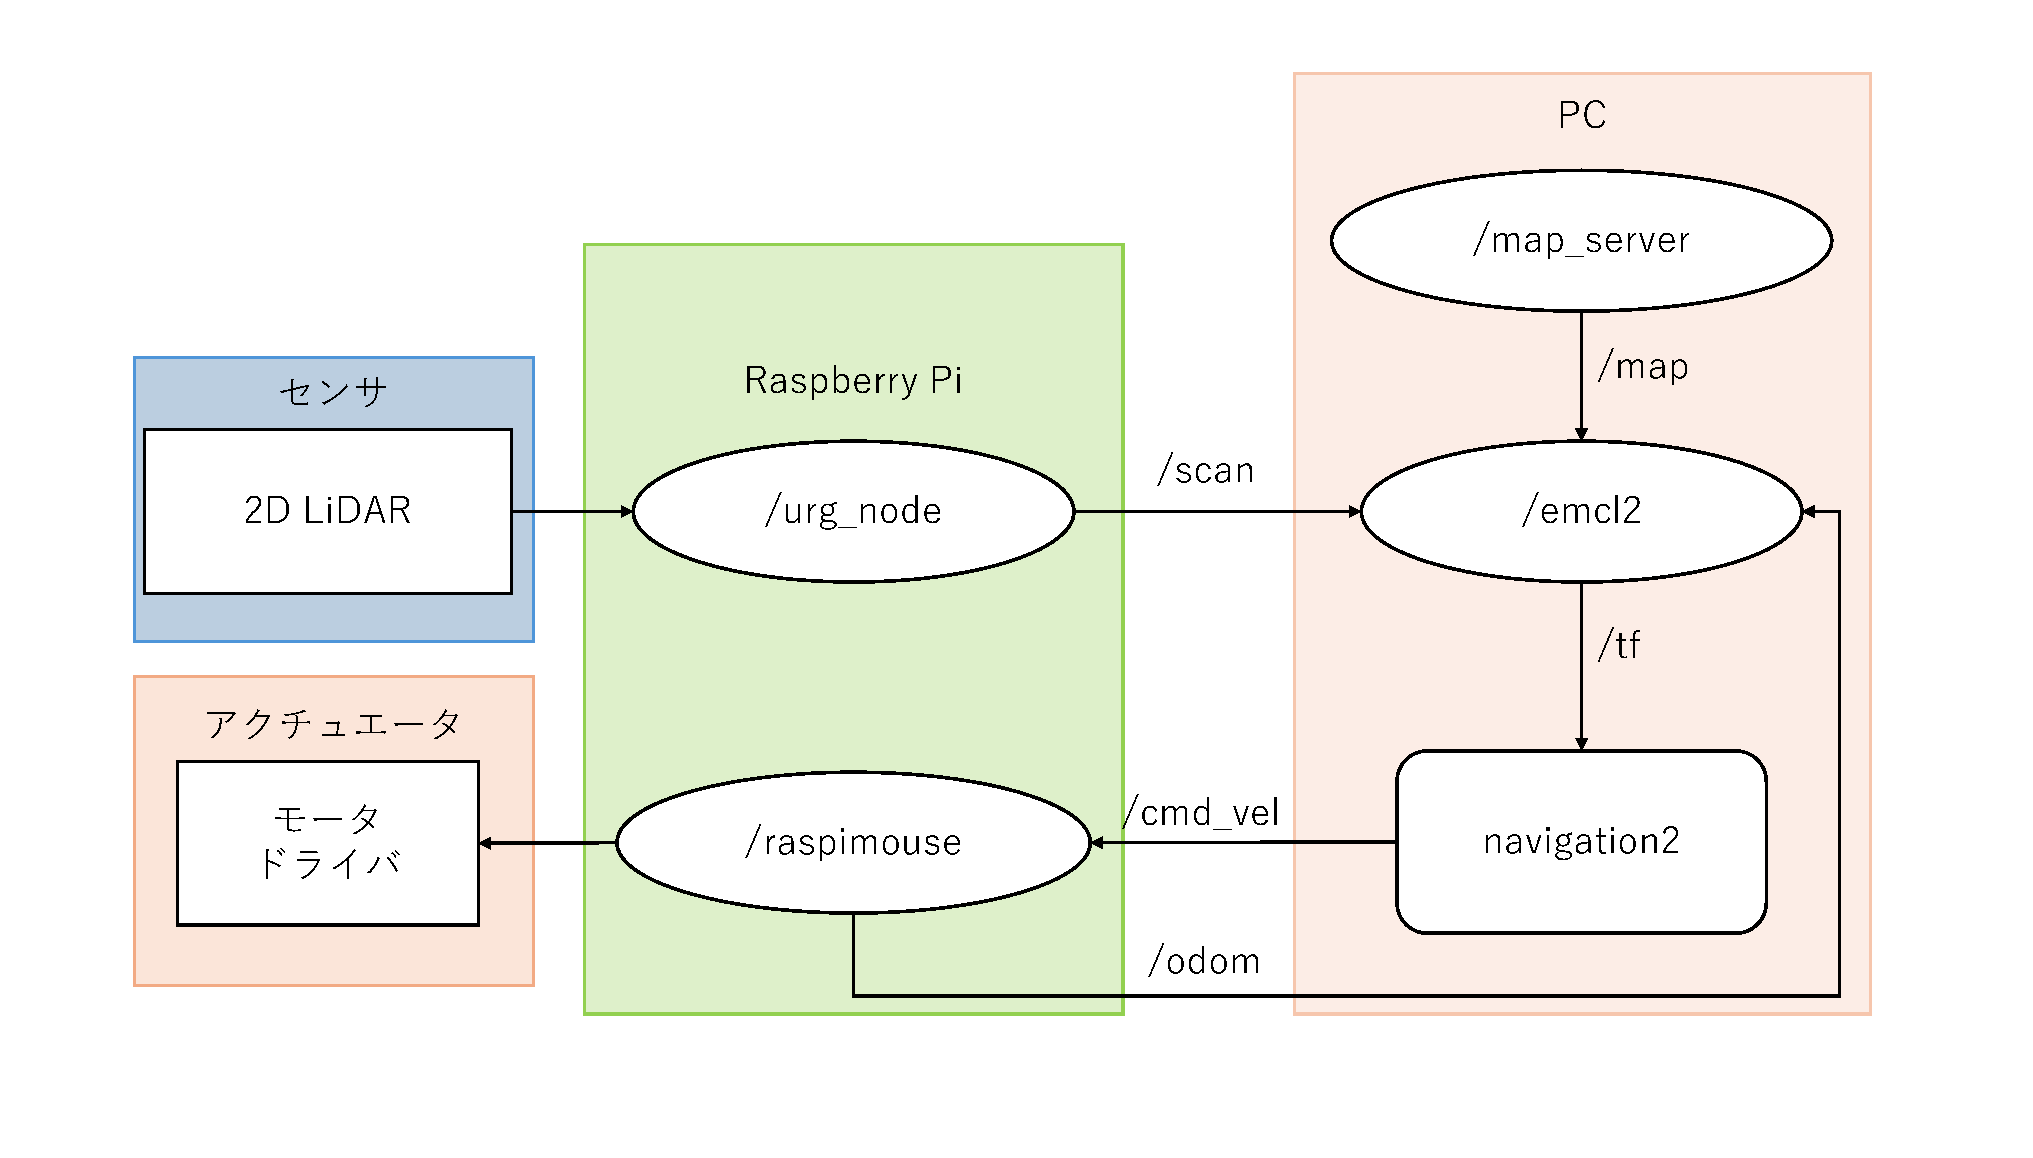
\includegraphics[width=1.0\linewidth]{figs/shiratama_system_diagram.eps}
    \caption{しらたまチームのシステム構成}
    \label{fig:shiratama_system}
  \end{center}
\end{figure}
